\chapter{Introducing Machine Learning}
%\label{sec:Methods}
\label{sec:ML}
In this chapter, we will introduce the different Machine Learning algorithms which are used in the analysis. 

The future of scientific experiments faces a problem: on one hand, we collect more data than we have ever done in the history of science. It opens up a whole new range of possibilities and increases the potential for new discoveries. On the other hand, the quantity of data is so vast that no human being, or group of human beings, could hope to sift through and analyze all the data in a single lifetime. However, it's not good enough to have a ``dumb'' computer algorithm sort through the data, since if the computer cannot adapt and pick out interesting features, a human would need to double check the results anyway. We need a technique that is both efficient and ``smart''. For this reason, and others, Machine Learning (ML) is fast becoming the standard way of analyzing data in science, and in high energy physics in particular. 

Indeed, compared to the cut and count method, ML techniques often provide a more efficient way to perform analyses. It can handle massive datasets and give results in a reasonable time frame. This is needed since the datasets have become increasingly large after each experimental upgrade at for example the LHC. The ML methods may be better at distinguishing between background and signal since they have the potential to pick up characteristics in the data which are difficult for a human to identify (because it might pick out characteristics in the data that a human would never notice), which we are trying to optimize in our analysis. The regular cut and count analysis is implemented by a person, and they analyze the data. For us, however, we will try to separate the signal from the background using ML algorithms. A discussion of these is presented in the following sections. 

Broadly speaking, an ML algorithm can be explained as shown in figure \ref{fig:MLex}. We have an input variable X that we send into an ML model of our choice, and we get the actual output Y (the ML output) and the predicted output Y' (the output we expect). Let us say that we give the ML model a variable with label 1; then the predicted value is 1 and the actual output will (hopefully) be either 1 or close to 1.   

\begin{figure}[H]
    \centering
    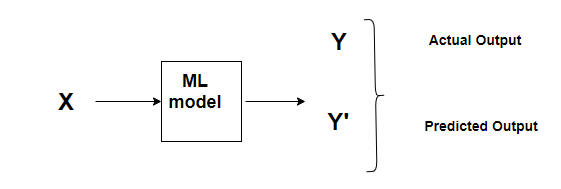
\includegraphics[width = \textwidth]{Figures/FromOnline/MLex.png}
    \caption{A very simple illustration of an ML algorithm \cite{MLex}.}
    \label{fig:MLex}
\end{figure}


\begin{comment}
In this thesis we are, as mentioned earlier, focusing on using ML algorithms to find new optimal cuts. This is just one of many ways of using ML in particle physics. Another way is to use it for anomaly detection of new particles. In that instance, we train our ML algorithm on background and then it will tell you if it have found something that is not behaving like the known backgrounds. \improvement{Dette hører kanskje heller hjemme i en evt outlook??}
\end{comment}


\section{Machine Learning basics}
In this thesis, we are focusing on using ML algorithms to separate the signal from the background. This is done by the ML algorithms called Boosted Decision Trees (BDT) and Neural Networks (NN). Before we go into the specifics, we will give a short introduction to some ML basics.

\subsection{Training and testing}
\label{sec:TandT}
To obtain our BDT and NN results, we have to split our datasets into training and test sets. We split the dataset into 2/3 for training and 1/3 for testing. It is common practice to divide the train and test set like this, but it is also possible to choose a smaller training set and a larger test set. The reason for doing this is that we want to check if our model is learning and is able to classify the background as background and the signal as signal - before we, in the end, give it actual data. 

\subsubsection{Validation test}
In addition to a standard test set, we need a validation set to avoid overtraining (this is not used to test whether the model works, but rather to prevent overfitting - see below). A validation set is a set which hasn't been used to train the algorithm. We use the validation set to see when the model cannot do better with calculating a validation loss, which is the loss for the validation set - and will be explained later in this chapter - for each epoch or estimator the network or BDT goes through. An epoch is the number of cycles the NN does the training and estimator is the number of the times we want to boost the tree. If the validation loss does not become better after e.g., ten steps, another function breaks the training before it has finished all of the epochs or estimators. This is done by a function called \textit{early stopping}, which stops the training. This is very useful for the NN and BDT since there is one less parameter we have to worry about, namely the epochs or estimators. We only have to set a value high enough for the model to get far enough through the training. 

\subsection{Overfitting and underfitting}
In ML we encounter a very common problem while training our model, namely overfitting and underfitting. The goal when training a model is to get it to fit the data as well as possible; but this training can't be too precise or the model will be useless if your data doesn't look exactly the same the next time you are using it. That would lead to loss of generality and our model would become dataset specific. This is overfitting. Underfitting is of course the opposite problem: the model is too simple to adapt to slightly more complex datasets, and the algorithm will simply use a simple function to fit data. These ideas are very well illustrated in figure \ref{fig:overunderfitting}. 

\begin{figure}[H]
    \centering
    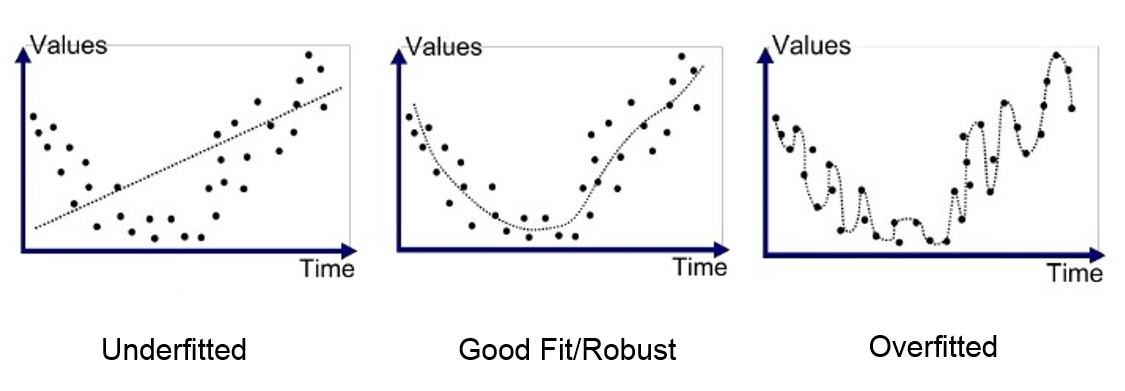
\includegraphics[width = \textwidth]{Figures/FromOnline/overunderfitting.png}
    \caption{An illustration of underfitting and overfitting \cite{overunderfittingpic}.}
    \label{fig:overunderfitting}
\end{figure}


The goal in our case is to optimize the ML model so that it efficiently can separate signal from background. If we overfit, it means that it can only find the signal for which we have trained on, and if it turns out that the new physics we are looking for is slightly different, our network will not be able to distinguish it from background. This is particularly important in our case since we train the network on simplified SUSY/DM models which we know are not the true realization of new physics in nature, but we believe that they have similar phenomenology. However, if we overtrain, our ML model will not be able to find any possible new physics in the data which looks slightly different from what we have trained on.

\subsection{Evaluating metrics}

\subsubsection{Accuracy}
In ML we have many ways to measure how well or badly our algorithm is performing; one of them is the \textit{accuracy} \cite{accuracy}. The accuracy expresses in percentage how accurate your algorithm is performing and can be calculated as

\begin{equation}
    \label{eq:acc}
    accuracy = \frac{correct}{correct + incorrect},
\end{equation}
where \textit{correct} is all data points that are classified as true positives (TP) and \textit{incorrect} as false positives (FP)\footnote{\textit{True positives} are all the datapoints that are correctly classified as positives, while \textit{false positives} are the datapoints which are classified as positive when they actually are negative. The same labeling holds for the negative classifications (TN/FN).}. This could be the only metric needed to evaluate a model; it gives a very basic measure on how, well, accurate - or reliable - the ML model is. 

\subsubsection{Loss and cost function}
Earlier we mentioned the validation loss, which is calculated for the whole training set during training. The loss is calculated for each estimator (BDT) and epoch (NN). The loss can be calculated in many different ways and we should choose the one best suited for the problem. In our case we want to classify the background and signal as two variables, namely 0 and 1. This means that we are looking at a binary classification problem and we can use a binary classification loss function \cite{Loss}, namely binary \textit{cross-entropy}. Mathematically it can be derived as follows. We have a true probability $p_i$ and a distribution of the predicted values $q_i$. The probability to get the outcome $y=1$ is given by

\begin{equation}
    \label{eq:prob1}
    q_{y=1} = \Hat{y} = g(\textbf{w} \cdot \textbf{x}) = \frac{1}{1+e^{-\textbf{w} \cdot \textbf{x}}},
\end{equation}
where $\textbf{x}$ is a vector of input features, $\textbf{w}$ is a vector of optimized weights and $g(\textbf{w} \cdot \textbf{x})$ is a logistic function.

To find the probability of $y=0$ we can write

\begin{equation}
    \label{eq:prob0}
    q_{y=0} = 1- \Hat{y}.
\end{equation}

This gives us the notation setup, $p \in \{y, 1-y\}$ and $q \in \{\Hat{y}, 1-\Hat{y}\}$ and we can get the difference between $p$ and $q$ by using the cross-entropy $H(p,q)$, which leads to

\begin{equation}
    \label{eq:crossentropy}
    H(p,q) = - \sum_i p_i \log q_i = - y log \Hat{y} - (1-y) log(1-\Hat{y})
\end{equation}

While we are training, logistic regression optimizes the log loss $J$\footnote{Here the loss function is called the cost function $J$. This might be a bit confusing because the cost function is defined as the loss function for all training sets, but in our case the loss and cost are the same.} which means that we optimize the cross-entropy in the sample. This is given by

\begin{equation}
    \label{eq:loss}
    J(\textbf{w}) = \frac{1}{N} \sum_{n=1}^N H(p_n, q_n) = - \frac{1}{N} \sum_{n=1}^N \big[y_n log \Hat{y}_n + (1-y_n) log(1-\Hat{y}_n)\big],
\end{equation}
where $\Hat{y}_n$ is defined by equation \ref{eq:prob1}.

Cross-entropy is the best loss function to use in our case and is the preferred function to use in similar cases. Ideally, the cross-entropy loss should be 0 during training - this corresponds to the minimum possible loss. In practice, this does not happen; in fact, a validation loss of 0 normally indicates a different problem  - likely overfitting. 


\subsubsection{ROC-curve and AUC-score}
To analyze our results from both ML algorithms, we are going to use the ROC-curve and the AUC-score, which is short for Receiver Operating Characteristic and Area Under Curve. AUC refers to the area under a ROC curve, and this curve is a plot of the True Positive Rate (TPR) against the False Positive Rate(FPR). TPR is the actual positives that are identified correctly, called \textit{signal efficiency}, and FPR is the rate between the negative events categorized as positive and the negative events. In figure \ref{fig:ROCAUCex}, we can see how this looks. 

\begin{figure}[H]
    \centering
    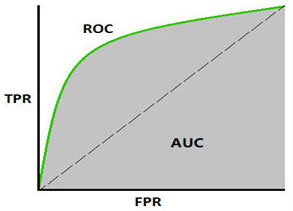
\includegraphics[width = 0.5\textwidth]{Figures/FromOnline/ROCAUC.jpg}
    \caption{An example of a ROC curve \cite{ROCAUC}.}
    \label{fig:ROCAUCex}
\end{figure}

If we look at the green line in figure \ref{fig:ROCAUCex}, which is changing from model to model, we can see it has a smooth curve. If the green line creates a right angle in the top left corner, we will get an AUC score of 1, meaning the ML algorithm classifies correctly every signal and background event. In other words, the algorithm picks correctly every time. If the green line follows the diagonal dashed line, the algorithm is correct approximately 50 \% of the time, which is statistically the same as having the model randomly classify objects. If the curve goes below the dashed line, the model classifies the background events as signal and the signal events as background, precisely the opposite of what we are trying to do. 










\begin{comment}
The use of machine learning (ML) is becoming the standard way of analysing data and interpreting various measurements and searches for new physics. ML is a more sophisticated method to do an analysis than the regular methods, such as the cut and count method. It is also usually more sensitive which gives us the opportunity to separate the signal from the background more efficiently than we do today.  We classify ML and specifically neural networks (NN) into two types, deep and shallow. Deep neural networks (DNN) is a NN with several hidden layers with quite few nodes/neurons in each layer. Shallow neural network (SNN) is a NN with only one hidden layer, but to obtain good results you need many more nodes/neurons in the hidden layer which gives us much more parameters to worry about. In this project we are going to concentrate on deep learning and compare the results with a simple SNN. 
\end{comment}


\section{Boosted Decision Trees}
\label{sec:BDT}

Boosted decision trees (BDT's) are one of the easiest ways to implement Machine Learning. It's typically not very sensitive to its hyperparameters, and is relatively easy to set up. In this thesis we have used XGBoost \cite{xgboostAbout}, which is one specific way to boost a decision tree. Before we explain boosted DTs however, we have to understand a regular DT.


\subsection{Decision Tree}

A decision tree is something we often do when thinking, even if we don't refer to the process as such. When we make a choice, we use a decision tree. Let us say that we have a picture of a person and we want to figure out if it is a boy or a girl. To make this conclusion we identify different features like whether the person has long hair, a beard, makeup, and so on. Then we set up a decision tree that will split our input data, which in this case is our picture, and make decisions based on the features you give it. Of course, we are not going to look on gender recognition in this thesis, but in principle decision trees can classify many things. This was just a small illustration of the simplicity and broad usage of BDT's.

Our goal is to use these principles to separate the signal from the background events. We give our decision tree some input data \cite{DTppt}, which consists of Monte Carlo (MC) simulated background and different signal samples (which are also obtained by MC simulations). Our decision tree will then split our data based on features we provide, e.g. invariant mass and missing transverse energy. 

\begin{figure}[H]
    \centering
    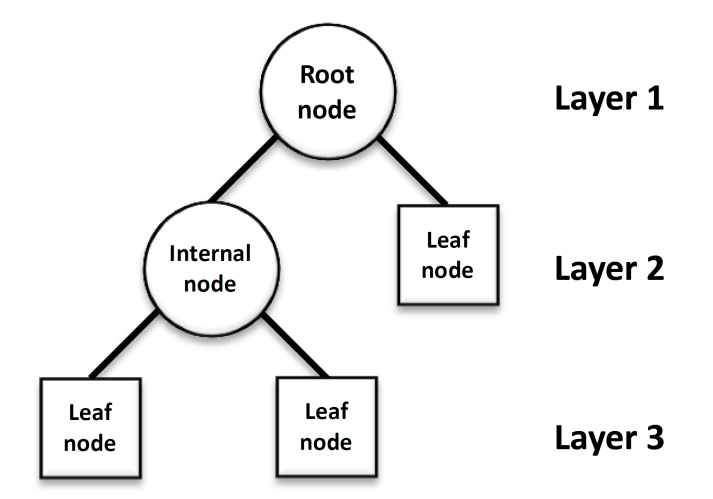
\includegraphics[width=0.5\textwidth]{Figures/FromOnline/Basic-structure-of-a-decision-tree-All-decision-trees-are-built-through-recursion.png}
    \caption{A sketch of how a decision tree is set up. \cite{DTpic}}
    \label{fig:DTpic}
\end{figure}

If we look at figure \ref{fig:DTpic}, we can see that we have three layers and three different types of nodes. The \textit{root node} is our input node, i.e. our input data, which for the first round is signal and background samples. Then the decision tree splits up our input data depending on the features we give it. This part will happen continuously through \textit{internal nodes} until we hit the depth of the tree, i.e. the last layer, or only have \textit{leaf nodes} left. As mentioned in section \ref{sec:TandT}, we split our input data into train and test parts where we save some data to test how well our model is trained. If we are happy with our results, we can test our pretrained model on real data and potentially extract some signal.


\subsection{Boosting}
Decision trees are weak learners (meaning that they typically perform badly), but if we ensemble several weak learners, we can get a strong learner. This process gives what it is called a boosted decision trees. Boosting creates a collection of predictors, which means that we fit consecutive trees, and at every step, we try to solve for the net error from the prior tree. If a hypothesis misclassifies the input, its weight will increase, so it would more likely classify it correctly next time. In figure \ref{fig:BDT}, we can see a sketched diagram of a BDT.


\begin{figure}[H]
    \centering
    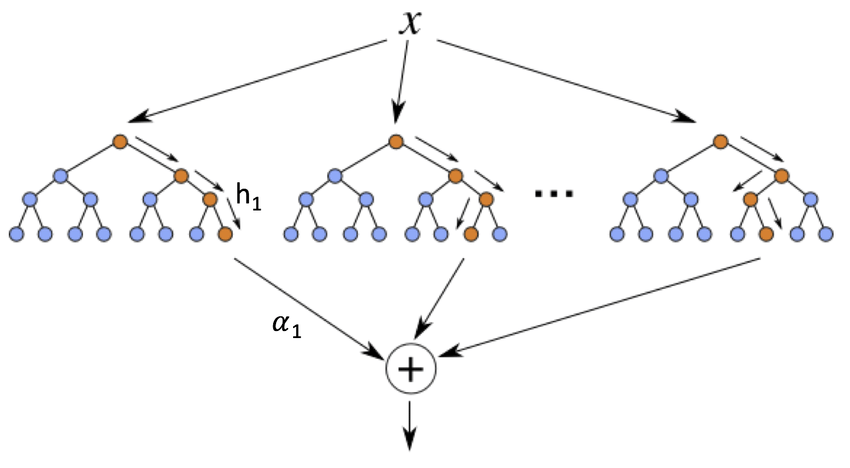
\includegraphics[width = 0.7\textwidth]{Figures/FromOnline/BDT.png}
    \caption{Illustration of a BDT \cite{BDTpic}.}
    \label{fig:BDT}
\end{figure}

There are many ways to boost a decision tree, but in this thesis we have used a Python software library called XGBoost \cite{xgboostAbout}, which is short for eXtreme Gradient Boosting. This library uses a gradient descent while boosting the decision trees. The gradient descent is an algorithm that can optimize the differential loss function, i.e., the next tree will try to recover the loss from the previous tree. Note that the loss is defined as the difference between actual and predicted values \cite{BDT}. 

XGBoost is optimized to be highly efficient and flexible \cite{xgboostAbout}. It is written in C++, but offers a user interface in python and other languages. In this thesis we are using a class in XGBoost called \texttt{XGBClassifier} which, as implied by the name, classifies the data. We give all our input data a label 0 or 1 for background and signal respectively and train our model, with the different features, on what should have label 0 or 1 in the end. This is what we call \textit{supervised learning} because we help our model by providing a label in the input. The \texttt{XGBClassifier} takes a lot of arguments, which can be found in the Scikit-Learn API reference guide \cite{xgboostargument}, but in this thesis we use just the ones that are necessary for our purpose. The arguments that we have used are mentioned in the analysis chapter.

\subsection{Feature importance}
We are also going to look at the feature importance in the analysis. This is a way to see which features were important while constructing our BDT. This is an interesting aspect of the analysis because this will change from process to process and we will also be able to see if it matters if we train on different signal samples or not.

\section{Neural networks}
\label{sec:NN}
Neural Networks (NN) are probably the most popular machine learning algorithms that we use today. This is also what is often used for face and speech recognition by companies like Google and Apple \cite{NNarticle}. NN does basically the same as a BDT, but instead of splitting the input data into background and signal at each node, each node is trained on different features. 

NN are a collection of nodes, like the ones we have in BDT. \ref{sec:BDT}. Instead of many trees with nodes, we are now creating a network with these nodes as we can see in figure \ref{fig:NN}. 


\begin{figure}[H]
    \centering
    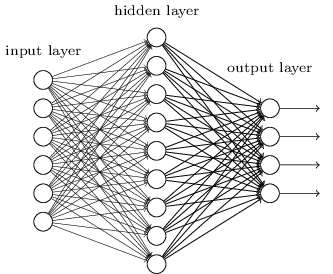
\includegraphics[width = 0.5\textwidth]{Figures/FromOnline/tikz35.png}
    \caption{Illustration of a neural network \cite{NNpic}.}
    \label{fig:NN}
\end{figure}

We can see that the network consists of one input layer, one hidden layer and one output layer. This is a very simple NN and is often called a \textit{shallow neural network} (SNN) since it has only one hidden layer. If we increase the number of hidden layers to two or more we have a deep neural network (DNN) as we can see in figure \ref{fig:DNN}

\begin{figure}[H]
    \centering
    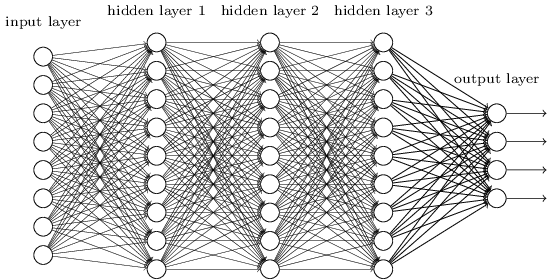
\includegraphics[width = 0.7\textwidth]{Figures/FromOnline/tikz36.png}
    \caption{Illustration of a deep neural network \cite{NNpic}.}
    \label{fig:DNN}
\end{figure}

In this thesis we have built a NN with a tool called \texttt{KerasClassifier}\footnote{Keras \cite{keras} is a NN library for Python.} which, as for the BDT, classifies the data. For our network to be able classify, we have to send in some pre-labeled data to train it. This is done by simply giving the background label 0 and signal label 1. Additionally, we have to understand what happens in the NN to know what parameters we should adjust in order to train and analyse the data. 

The NN has many more dependencies than the BDT. It is therefore unfortunately more sensitive to possible under- and overtraining, but for correct composition of parameters, it will typically be better trained than a BDT. To achieve the optimal results, we need a lot of computing power and time to optimize. 

There are many advantages and disadvantages with both SNN and DNN but it is in principle possible to achieve the same results with both. In a SNN you can increase the number of nodes and get the same results as for a DNN with several layers and fewer nodes in each layer. The problem with doing it that way is that we get more free parameters by increasing the number of nodes, which again increases the possibility that our model gets biased and hence over or underfits.

This is unfortunately not as trivial as for a BDT, but maybe easier to adapt to different purposes. In our case we are going to use it to distinguish signal from background.

With the basics in place, we can now describe NNs in more detail. Next we provide an overview of the activation function, how the network evolves, and how it gets better with training.

\subsection{Activation functions}
To get the output for the different nodes in a layer, we need an activation function. This output is again used as input for the next layer until you reach the last layer, which then will give us our final output/results.

Since Machine Learning doesn't come from a theoretical prediction which is implemented numerically, the choice of activation function for different problems is found by trial and error. The activation function will provide a number between 0 and 1 \cite{AF}, which is sent into the next nodes in the next layer. Some activation functions provide a number between -1 and 1 instead, but this depends on how the activation function we choose behaves, as we can see in figure \ref{fig:activations}. In the next sections we are going to look more closely at the different activation functions we have used in this thesis. We are also going to consider some other activation functions that are not used in this thesis but still of very common use in ML.


%In the network, each node uses an activation function to send the total input in that node as a number between 0 and 1 to the next layer. Tanh gives a number between -1 and 1.

\begin{figure}[H]
    \centering
    \begin{subfigure}[t!]{0.3\textwidth}
    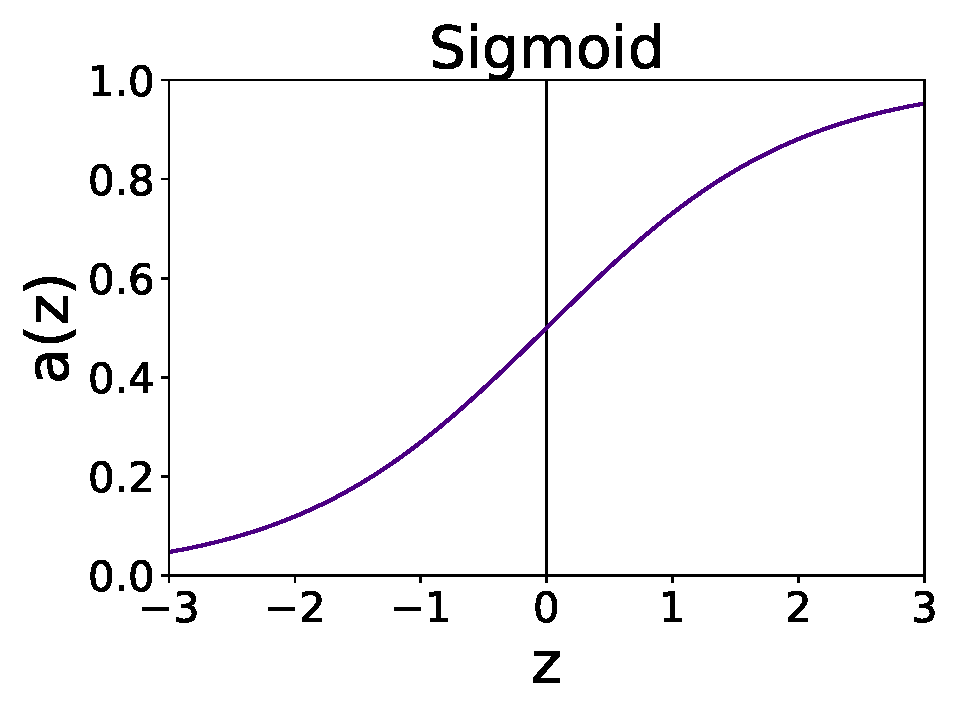
\includegraphics[width=\textwidth]{Figures/sigmoid.pdf}
    \caption{}
    \label{fig:sigmoid}
    \end{subfigure}
    \begin{subfigure}[t!]{0.3\textwidth}
    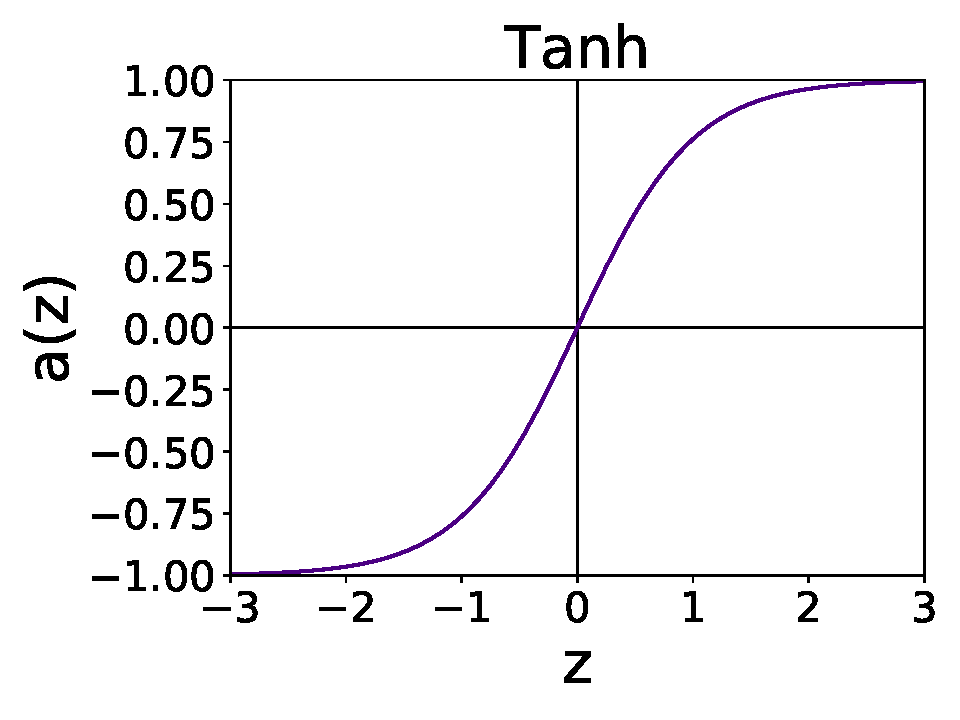
\includegraphics[width=\textwidth]{Figures/tanh.pdf}
    \caption{}
    \label{fig:tanh}
    \end{subfigure}
    \begin{subfigure}[t!]{0.3\textwidth}
    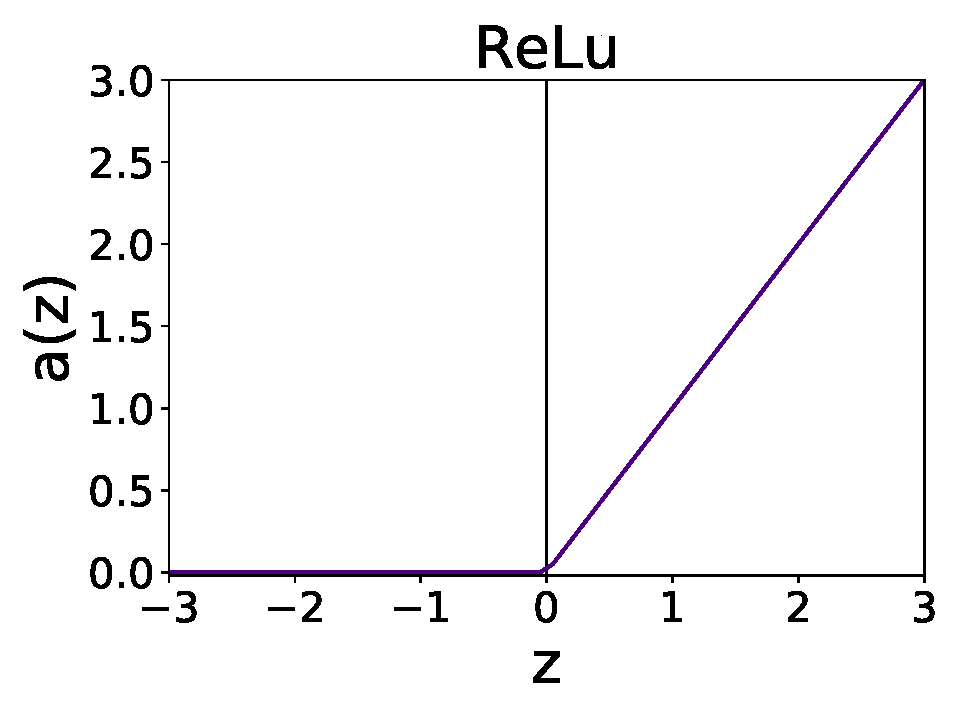
\includegraphics[width=\textwidth]{Figures/relu.pdf}
    \caption{}
    \label{fig:relu}
    \end{subfigure}
    \caption{This is an illustration of the behaviour of three different activation functions. In (a) we can see the Sigmoid function, in (b) the Tanh function, and in (c) the ReLU function.}
    \label{fig:activations}
\end{figure}



\textbf{Sigmoid}

The Sigmoid function, figure \ref{fig:sigmoid}, is a logistic activation function and is given by equation \ref{eq:sigmoid} below.

\begin{equation}
    \label{eq:sigmoid}
    a_i = \frac{1}{1+e^{(-z_i)}},
\end{equation}

where $z_i$ is the output value from the i-th node in the output layer.

As we can see in figure \ref{fig:sigmoid}, the Sigmoid function gives us a value between 0 and 1. This makes this activation function a good choice if we have to predict a probability for the output. A drawback, and the reason we have to use other activation functions sometimes, is that the Sigmoid can get the NN stuck on its training time because of the calculation time of the exponential. This is not an optimal activation function to use inside the network, but in the output layer it is the preferred one. We want our network to classify our output as signal or background which we have labeled as 1 and 0. 


\textbf{Tanh (Hyperbolic tangent)}

In addition to the Sigmoid function we have the tanh function, figure \ref{fig:tanh}, which is shaped the same way as the Sigmoid function, but it gives values between -1 and 1 instead of between 0 and 1. This we can see in figure \ref{fig:tanh} and it is given by equation \ref{eq:tanh} below.

\begin{equation}
\label{eq:tanh}
a_i = \tanh(z_i)
\end{equation}

Since we also can get negative numbers from this activation function, it is preferred instead of the Sigmoid if we have negative numbers in the input. This function returns negative values as negative unlike e.g. Sigmoid which only returns 0 or 1. Since we don't care for negative values in our case, this activation function is not used in this thesis. 

\textbf{ReLU (Rectified Linear Unit)}

One of the most popular activation functions is the ReLU function. This function outputs 0 for any negative value, and if the value is positive, the function returns the value as it is. This is shown in figure \ref{fig:relu}. Since all data that is below zero becomes zero, it can be hard do get a good read out of the data because the data may sometimes assume negative values. The ReLU function is given by equation \ref{eq:relu}.

\begin{equation}
\label{eq:relu}
    a_i = max(0,z_i).
\end{equation}

Since we're not interested in negative values we are using this activation function in our hidden layers. The Sigmoid function would also be a good choice when we are thinking about our wanted form of the output. But, as mentioned earlier, it can get stuck in its training time.

\textbf{Other activation functions}

The three functions mentioned above are not the only activation functions one can use. Since every problem has different approaches, we have to adjust these functions for our needs. There are, for example, many different adjustments done with the ReLU function to get a better activation output in problems that need adjustment to perform optimally. One of the newest activation functions is called Swish \cite{Swish}, which is simply a modification of the Sigmoid function given by equation \ref{eq:swish}. 

\begin{equation}
    \label{eq:swish}
    a(x) = x \cdot Sigmoid(x)
\end{equation}

The developers of the Swish function state that it does overall a better job than the widely used ReLU function, but until this time there is no evidence in literature supporting this claim. As such, we will stick with ReLU in this thesis. 

\subsection{Feed forward and back propagation} 
Every node in the neural network has an activation function connected to itself and if the node is connected to another node it also has a weight for each node it is connected to. To create the new node we simply multiply the nodes activation with the weight and sum them together like so

\begin{equation}
    a_1 \cdot w_1 + .. + a_n \cdot w_n = \text{new node}
\end{equation}

This operation is done for every node in every layer, and fed to the next layer until we hit the the output layer. This is what we call \textit{feed forward} because we always send the obtained information forward from input to output layer.

We also have a method to go back in the network to optimize it, namely \textit{back propagation}. What we do is go back to the previous layers to optimize the weights. This is not what we call an optimizer and should not be confused with that; it's merely the process of going backwards. Back propagation is probably the most important step in a NN, because this optimizes our model and makes sure that our training goes well. 

\subsection{Optimizers}

When training a NN, we need to know how well it performs during and after the training. For this we use a loss function $L$. There are many different types of functions that are used, depending on what we want to do with the network.

We want to minimize the loss function to make the prediction error as small as possible, i.e. optimize the network. And to do this, we use an optimizer.

\subsubsection{Stochastic Gradient Descent\cite{training_model}}

The gradient descent method uses the fact that a function $F(x)$, where $x = (x_1,x_2,...,x_n)$, will increase fastest in the direction of the gradient of the function, $\nabla F$. We want to move in the opposite direction of the gradient to make sure that we decrease the loss function.

We then multiply this gradient with a number $\eta$ called "the learning rate", and subtract this from the current weights $w_j$. In the case of neural networks, $F(x)$ is the loss function $L$. This leads to equation \ref{eq:w_update} 

\begin{equation}
    w_j = w_j - \eta\frac{\partial L}{\partial w_j}
    \label{eq:w_update}
\end{equation}

To speed up the training we can also add a stochastic part to the method, which means that we randomly choose a batch size of the data that we use to approximate the derivative, and use that to update the weights. This is also called Mini Batch Gradient Descent. 

The data that we want to use might be very noisy, so we can use a technique to de-noise the data \cite{SGD_momentum}. This is done by adding a momentum, which is a moving average of our gradients. We now subtract this from the weights. The equations now become 

\begin{equation}
    V_i = \beta V_i + (1 - \beta)\nabla_w L
    w_i = w_i - \eta V_i
    \label{eq:momentum}
\end{equation}

One way to look at this last addition is viewing the movement in parameter space as an object that moves one step at a time downhill. When we add momentum, it is like giving this object some physical momentum. Now when the object finds the minimum, it will continue a little bit back and forth to make sure it has found the minimum. A good reason to add this is if there are many saddle-points where the optimizer might stop. With momentum, it will move past, and then continue the descent on the other side without stopping.

\subsubsection{Adam\cite{Goodfellow-et-al-2016}}

The learning rate is one of the most difficult parameters to optimize, because any change to its value may have a huge impact on a method's performance. To circumvent this, we can use a method that has an adaptive learning rate. 

Adam is currently the most popular optimization algorithm today, and the name is derived from Adaptive Moments. It is an update to another optimization algorithm called RMSProp, which stands for Root Mean Square Propagation. RMSProp uses the running average of recent gradient magnitudes, and divides the learning rate by this average. This is done for every weight in the NN.

Adam takes this a step further. It uses an estimation of the first-order moments of the gradient as momentum, and also adds a bias correction to both the momentum and the second-order moments.

